% !TEX root = ../../seminar.tex

\subsubsection{Research Question}

The question the later study is designed to answer is called research question \cite{Vickers}. It should be an answerable question and address a relevant issue in the research area \cite{Dyba2005}. Preceding a research question is the need for a deep understanding of the topics that have already been studied, in order to produce questions which drive knowledge further. The questions that arise during the acquisition of knowledge, and cannot be answered by means of EBSE, are likely appropriate questions for further research \cite{Farrugia2009}.

There are two general classes of research questions: qualitative and quantitative questions. Qualitative research states questions which report, describe, or explore a subject \cite[p. 139-141]{Creswell2014}. The issues computer science students are confronted with are often of quantitative nature than of qualitative (e.g. Is databese engine X faster than database engine Y?). These problems are different from what researchers commonly investigate (see issue \ref{itm:issue7} in table \ref{table:issuesEBSE}) \cite{Rainer2006}. Therefore, focus is on quantitative research questions in this paper. \q{Quantitative research questions inquire about the relationships among variables} \cite[p. 143]{Creswell2014}, and from them emerge quantitative hypotheses.

To understand the structure of research questions Shaw provides a model where she categorizes research questions from software engineering papers in five types \cite{Shaw2002} \todosoft{(maybe cut out)}. 

To design a good research question Haynes coined the acronym PICO: Population, Intervention, Comparison group, and Outcome \cite{BrianHaynes2006}. Sometimes Time is added as fifth component, when it is important over what time frame the study is conducted, see left box in figure \ref{fig:PICOT_FINER}. A research question structured with the PICOT approach supports in restricting the research question and steers thereby hypotheses and study. By restricting the research question researchers can limit bias and increase the internal validity of the study, but a too narrow question may also lead to decreased external validity \cite{Farrugia2009}. 

Before PICOT Sackett and colleagues suggested that good research questions consist out of three components: Intervention, Context and Outcome \cite{Sackett2000}, which is a more coarse grained decomposition than PICOT. Dyb{\aa} \etal displayed a fitting example for this template in software engineering: \q{Does pair programming lead to improved code quality when practiced by professional software developers?} \cite[p. 60]{Dyba2005} Here the intervention (technology) is pair programming, the context of interest are professional software developers, and the outcome (effect) is improved code quality \cite{Dyba2005}. To verify the quality of a freshly designed research question Hulley \etal suggest the use of the FINER criteria. It highlights key aspects of the question and provides thereby new angles to view the proposed study from. The FINER criteria consists of: Feasible, Interesting, Novel, Ethical, and Relevant \cite{Farrugia2009}. A more detailed view of the FINER criteria can be seen in the right box of figure \ref{fig:PICOT_FINER}. \todosoft{specify more tips for writing a good question. Creswell2014)}  

\begin{figure}
	\centering
	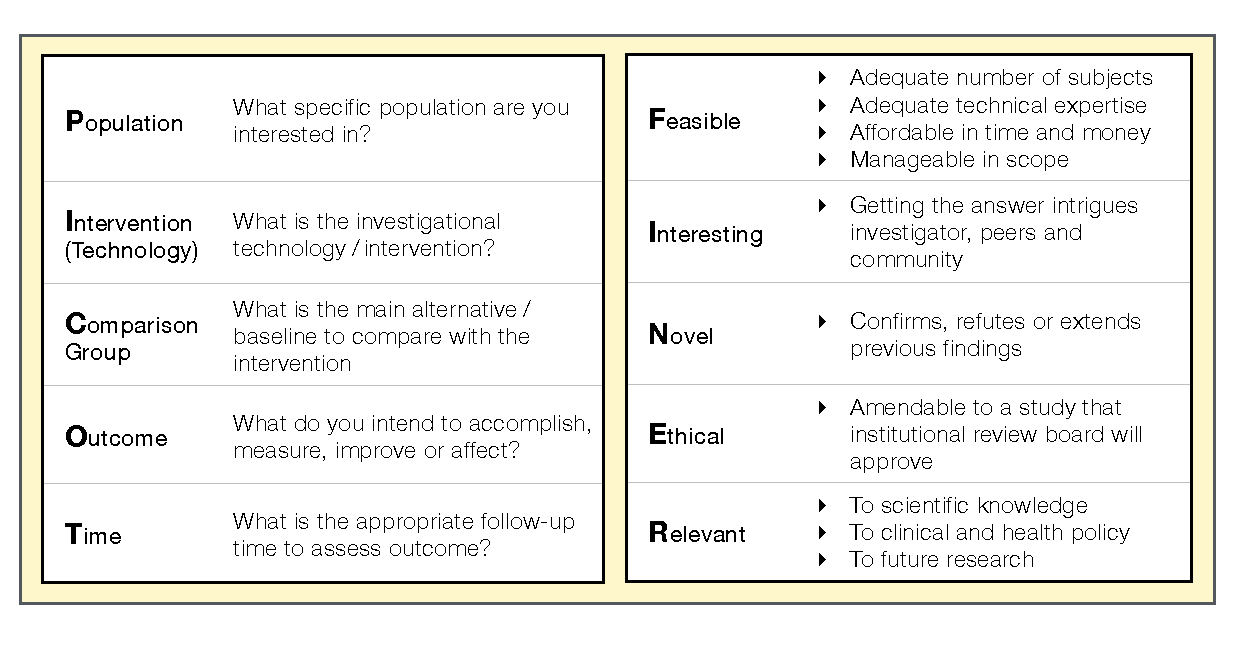
\includegraphics[width=12cm]{figures/picot_finer.pdf}
	\caption{PICOT criteria adjusted to fit better in computer science research \cite{Farrugia2009} and FINER criteria for a good research question \cite{Farrugia2009}.}
	\label{fig:PICOT_FINER}
\end{figure}

